% Options for packages loaded elsewhere
\PassOptionsToPackage{unicode}{hyperref}
\PassOptionsToPackage{hyphens}{url}
\PassOptionsToPackage{dvipsnames,svgnames,x11names}{xcolor}
%
\documentclass[
  letterpaper,
  DIV=11,
  numbers=noendperiod]{scrartcl}

\usepackage{amsmath,amssymb}
\usepackage{iftex}
\ifPDFTeX
  \usepackage[T1]{fontenc}
  \usepackage[utf8]{inputenc}
  \usepackage{textcomp} % provide euro and other symbols
\else % if luatex or xetex
  \usepackage{unicode-math}
  \defaultfontfeatures{Scale=MatchLowercase}
  \defaultfontfeatures[\rmfamily]{Ligatures=TeX,Scale=1}
\fi
\usepackage{lmodern}
\ifPDFTeX\else  
    % xetex/luatex font selection
\fi
% Use upquote if available, for straight quotes in verbatim environments
\IfFileExists{upquote.sty}{\usepackage{upquote}}{}
\IfFileExists{microtype.sty}{% use microtype if available
  \usepackage[]{microtype}
  \UseMicrotypeSet[protrusion]{basicmath} % disable protrusion for tt fonts
}{}
\makeatletter
\@ifundefined{KOMAClassName}{% if non-KOMA class
  \IfFileExists{parskip.sty}{%
    \usepackage{parskip}
  }{% else
    \setlength{\parindent}{0pt}
    \setlength{\parskip}{6pt plus 2pt minus 1pt}}
}{% if KOMA class
  \KOMAoptions{parskip=half}}
\makeatother
\usepackage{xcolor}
\setlength{\emergencystretch}{3em} % prevent overfull lines
\setcounter{secnumdepth}{5}
% Make \paragraph and \subparagraph free-standing
\ifx\paragraph\undefined\else
  \let\oldparagraph\paragraph
  \renewcommand{\paragraph}[1]{\oldparagraph{#1}\mbox{}}
\fi
\ifx\subparagraph\undefined\else
  \let\oldsubparagraph\subparagraph
  \renewcommand{\subparagraph}[1]{\oldsubparagraph{#1}\mbox{}}
\fi


\providecommand{\tightlist}{%
  \setlength{\itemsep}{0pt}\setlength{\parskip}{0pt}}\usepackage{longtable,booktabs,array}
\usepackage{calc} % for calculating minipage widths
% Correct order of tables after \paragraph or \subparagraph
\usepackage{etoolbox}
\makeatletter
\patchcmd\longtable{\par}{\if@noskipsec\mbox{}\fi\par}{}{}
\makeatother
% Allow footnotes in longtable head/foot
\IfFileExists{footnotehyper.sty}{\usepackage{footnotehyper}}{\usepackage{footnote}}
\makesavenoteenv{longtable}
\usepackage{graphicx}
\makeatletter
\def\maxwidth{\ifdim\Gin@nat@width>\linewidth\linewidth\else\Gin@nat@width\fi}
\def\maxheight{\ifdim\Gin@nat@height>\textheight\textheight\else\Gin@nat@height\fi}
\makeatother
% Scale images if necessary, so that they will not overflow the page
% margins by default, and it is still possible to overwrite the defaults
% using explicit options in \includegraphics[width, height, ...]{}
\setkeys{Gin}{width=\maxwidth,height=\maxheight,keepaspectratio}
% Set default figure placement to htbp
\makeatletter
\def\fps@figure{htbp}
\makeatother
\newlength{\cslhangindent}
\setlength{\cslhangindent}{1.5em}
\newlength{\csllabelwidth}
\setlength{\csllabelwidth}{3em}
\newlength{\cslentryspacingunit} % times entry-spacing
\setlength{\cslentryspacingunit}{\parskip}
\newenvironment{CSLReferences}[2] % #1 hanging-ident, #2 entry spacing
 {% don't indent paragraphs
  \setlength{\parindent}{0pt}
  % turn on hanging indent if param 1 is 1
  \ifodd #1
  \let\oldpar\par
  \def\par{\hangindent=\cslhangindent\oldpar}
  \fi
  % set entry spacing
  \setlength{\parskip}{#2\cslentryspacingunit}
 }%
 {}
\usepackage{calc}
\newcommand{\CSLBlock}[1]{#1\hfill\break}
\newcommand{\CSLLeftMargin}[1]{\parbox[t]{\csllabelwidth}{#1}}
\newcommand{\CSLRightInline}[1]{\parbox[t]{\linewidth - \csllabelwidth}{#1}\break}
\newcommand{\CSLIndent}[1]{\hspace{\cslhangindent}#1}

\KOMAoption{captions}{tableheading}
\makeatletter
\makeatother
\makeatletter
\makeatother
\makeatletter
\@ifpackageloaded{caption}{}{\usepackage{caption}}
\AtBeginDocument{%
\ifdefined\contentsname
  \renewcommand*\contentsname{Table of contents}
\else
  \newcommand\contentsname{Table of contents}
\fi
\ifdefined\listfigurename
  \renewcommand*\listfigurename{List of Figures}
\else
  \newcommand\listfigurename{List of Figures}
\fi
\ifdefined\listtablename
  \renewcommand*\listtablename{List of Tables}
\else
  \newcommand\listtablename{List of Tables}
\fi
\ifdefined\figurename
  \renewcommand*\figurename{Figure}
\else
  \newcommand\figurename{Figure}
\fi
\ifdefined\tablename
  \renewcommand*\tablename{Table}
\else
  \newcommand\tablename{Table}
\fi
}
\@ifpackageloaded{float}{}{\usepackage{float}}
\floatstyle{ruled}
\@ifundefined{c@chapter}{\newfloat{codelisting}{h}{lop}}{\newfloat{codelisting}{h}{lop}[chapter]}
\floatname{codelisting}{Listing}
\newcommand*\listoflistings{\listof{codelisting}{List of Listings}}
\makeatother
\makeatletter
\@ifpackageloaded{caption}{}{\usepackage{caption}}
\@ifpackageloaded{subcaption}{}{\usepackage{subcaption}}
\makeatother
\makeatletter
\@ifpackageloaded{tcolorbox}{}{\usepackage[skins,breakable]{tcolorbox}}
\makeatother
\makeatletter
\@ifundefined{shadecolor}{\definecolor{shadecolor}{rgb}{.97, .97, .97}}
\makeatother
\makeatletter
\makeatother
\makeatletter
\makeatother
\ifLuaTeX
  \usepackage{selnolig}  % disable illegal ligatures
\fi
\IfFileExists{bookmark.sty}{\usepackage{bookmark}}{\usepackage{hyperref}}
\IfFileExists{xurl.sty}{\usepackage{xurl}}{} % add URL line breaks if available
\urlstyle{same} % disable monospaced font for URLs
\hypersetup{
  pdftitle={Survival Compass},
  pdfauthor={Lexi Knight},
  colorlinks=true,
  linkcolor={blue},
  filecolor={Maroon},
  citecolor={Blue},
  urlcolor={Blue},
  pdfcreator={LaTeX via pandoc}}

\title{Survival Compass\thanks{Code and data are available at:
https://github.com/LexiKnight/Lung\_Cancer/tree/main}}
\usepackage{etoolbox}
\makeatletter
\providecommand{\subtitle}[1]{% add subtitle to \maketitle
  \apptocmd{\@title}{\par {\large #1 \par}}{}{}
}
\makeatother
\subtitle{Statistical Insights into Lung Cancer Patients Journey Post
Diagnosis}
\author{Lexi Knight}
\date{April 5, 2024}

\begin{document}
\maketitle
\begin{abstract}
This study investigates the impact of pathogenic stage and treatment
modalities on lung cancer survival post-diagnosis. Analysis of patient
data reveals significant correlation between pathogenic stage, seeking
treatment and survival outcomes. Notably, patients at advanced stages
with metastases in distant sites beyond the lung, extensive lymph node
involvement and tumors with extensive growth, invading nearby structures
demonstrate lower survival rates. These findings underscore the critical
importance of early detection, tailored treatment strategies and ongoing
research efforts to enhance lung cancer survival rates globally.
\end{abstract}
\ifdefined\Shaded\renewenvironment{Shaded}{\begin{tcolorbox}[frame hidden, borderline west={3pt}{0pt}{shadecolor}, enhanced, interior hidden, breakable, sharp corners, boxrule=0pt]}{\end{tcolorbox}}\fi

\hypertarget{introduction}{%
\section{Introduction}\label{introduction}}

Clinging to life amidst the shadows of lung cancer, where every breath
becomes a battleground. Survival becomes not just a statistic but an
interplay between several individual characteristics. We explore the
hidden keys to defying the odds and emerging victorious against one of
the deadliest adversaries of our time. Lung cancer is the leading cause
of cancer-related deaths in the world (Park, 2017). It is a disease that
develops in the lining of the airways in lung tissues. Non-small cell
lung cancer (NSCLC) is the most common type, accounting for 80-85\% of
all lung cancers according to the American Cancer society (Markman,
2023). Staging is important for prognosis and making treatment
decisions. Common treatments include surgery, radiation therapy and
chemotherapy (Kai, 2021). Pathogenic stage is determined by presence of
nearby metastasis, lymph node involvement as well as tumor spread and
size (Markman, 2023). This paper investigates the relationship between
lung cancer patients' survival and pathogenic stage. The estimand is the
median survival time in days post-diagnosis. We also look at whether
patients decided to have treatment and if so, which method; radiation
therapy or chemotherapy. Through analysis of a dataset made up of 981
patients in Sydney, Australia, we offer insight into the prognostic
markers.

Tumor size is often the main determinant of stage and treatment. As
tumor categories increase, the tumor expands, invading nearby structures
(Zhang, 2015). A study involving 52,287 patients diagnosed between the
years 1998 and 2003 found tumor size to be an independent prognostic
factor in estimating overall survival. The authors found that patients
presenting with larger tumors predicted a worse prognosis and thus are
associated with a decrease in survival. There is a similar relationship
between extensive lymph node involvement and patient survival (Zhang,
2015). Initial spread of cancer cells are localized, then become
regional, involving nearby lymph nodes and the most severe cases
comprises expansion to other organs such as the brain, liver and bones
(Markman, 2023). A study looked at five year survival rates based on the
severity of spread. 62.8\% of patients with localized spread, 34.8\% of
patients with regional and 8\% of patients with distant, advanced spread
were found to survive for 5 years post diagnosis. More than half of
these lung cancer patients have advanced spread to other organs when
diagnosed(Markman, 2023). Overall, it is found that patients with no
regional lymph node metastases, and smaller tumors are easier to be
treated and thus are associated with improved survival rates (Zhang,
2015).

Presence of metastatic LN is one of the most important determinants of
prognosis of NSCLC cases (Kai, 2021). In the early stage, cancer has not
spread to lymph nodes. As severity increases, lymph node metastasis
sequentially spreads to more distant lymph nodes such as mediastinal and
there is severe lymph node involvement (Park, 2017). Lymph node
involvement, also termed lymph node ratio, is a crucial factor in
guiding treatment options (Kai, 2021). A study made up of 97 patients
with a mean age of 63 who have undergone surgery between the years 2009
and 2015 in Korea find that increased lymph node involvement is
associated with a more advanced disease status and hence affiliated with
prognosis (Park, 2017). Another study looked at 11,341 NSCLC patients
between the years 2004 to 2015, from 18 geographically diverse
populations, covering approximately 28\% of the population of the United
States. These patients were treatment naive and underwent surgical
resection of the tumor. Although 5757 patients died, the rest showed
great results, with a median survival of 22 months (Kai, 2021). The
authors found that patients with low lymph node involvement lead to
higher survival compared to patients with high lymph node ratios. A
regression analysis revealed that lymph node ratio is an independent and
significant predictor of patient survival. The authors also observed
that disease burden and anatomical location of the lymph nodes involved
may influence the patients survival (Kai, 2021).

After tumor size, LN involvement and presence of distant metastasis are
categorized, the pathogenic stage of the cancer is then determined
(Eldridge, 2022). The most valuable prognostic factor in non-small cell
lung cancer is the pathogenic stage (Park, 2017) .Stage is determined by
tumor size, number of tumors and where the cancer has spread. Stage 1 is
localized spread, stage 2 and 3 is regional spread while stage 4 is
distant spread of the tumor (Eldridge, 2022). Cancer stage was
determined using the seventh American Joint Committee on Cancer staging
system (AJCC) (Park, 2017). A study done in Australia including 2119
lung cancer patients illustrated those with stage IV disease, the most
advanced stage, showed shorter survival than those at lower stages
(Denton, 2016). The earlier the cancer is found, that is the lower the
pathogenic stage, the greater the likelihood curative radiation therapy
is an effective treatment (Eldridge, 2022). However, there is minimal
literature looking at post-diagnosis survival rates based on pathogenic
stage and method of treatment. The extent of this disease illustrates
the importance of living a healthy lifestyle, undergoing regular
screening and development of improved treatment methods. Over the past
decade, there has been great improvement of lymph node assessment in
cancer patients (Kai, 2021). Experts hope survival rates continue to
improve with new therapies and treatment approaches (Markman, 2023).

The remainder of this paper is structured as follows. In
Section~\ref{sec-data}, we visualize the exploration of variables
constituting the pathogenic stage and treatment types.
Section~\ref{sec-model}, outlines the model employed to analyze the
relationship between these variables and the duration of survival
post-diagnosis. Moreover, Section~\ref{sec-results} offers visual
depictions of the study's outcomes. Finally, in
Section~\ref{sec-discussion}, we summarize the primary findings, propose
avenues for enhancement, and identify potential areas for future
research.

\hypertarget{sec-data}{%
\section{Data}\label{sec-data}}

Our data is

\begin{verbatim}
Warning: package 'ggplot2' was built under R version 4.2.3
\end{verbatim}

\begin{verbatim}
Warning: package 'dplyr' was built under R version 4.2.3
\end{verbatim}

\begin{verbatim}

Attaching package: 'dplyr'
\end{verbatim}

\begin{verbatim}
The following objects are masked from 'package:stats':

    filter, lag
\end{verbatim}

\begin{verbatim}
The following objects are masked from 'package:base':

    intersect, setdiff, setequal, union
\end{verbatim}

\begin{verbatim}
Warning: package 'showtext' was built under R version 4.2.3
\end{verbatim}

\begin{verbatim}
Loading required package: sysfonts
\end{verbatim}

\begin{verbatim}
Warning: package 'sysfonts' was built under R version 4.2.3
\end{verbatim}

\begin{verbatim}
Loading required package: showtextdb
\end{verbatim}

\begin{verbatim}
Warning: package 'showtextdb' was built under R version 4.2.3
\end{verbatim}

\begin{verbatim}
Warning: package 'arrow' was built under R version 4.2.3
\end{verbatim}

\begin{verbatim}

Attaching package: 'arrow'
\end{verbatim}

\begin{verbatim}
The following object is masked from 'package:utils':

    timestamp
\end{verbatim}

\begin{figure}

{\centering 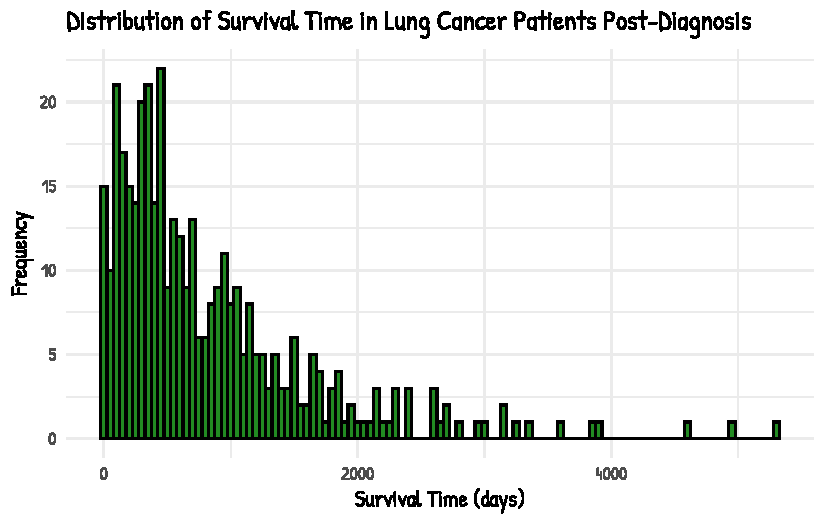
\includegraphics{paper_files/figure-pdf/fig-bills-1.pdf}

}

\caption{\label{fig-bills-1}bb}

\end{figure}

\begin{figure}

{\centering 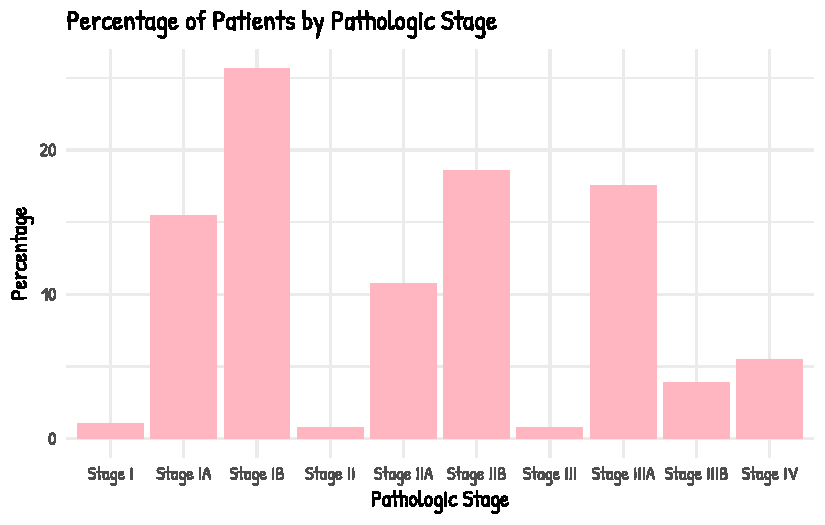
\includegraphics{paper_files/figure-pdf/fig-bills-2.pdf}

}

\caption{\label{fig-bills-2}bb}

\end{figure}

\begin{figure}

{\centering 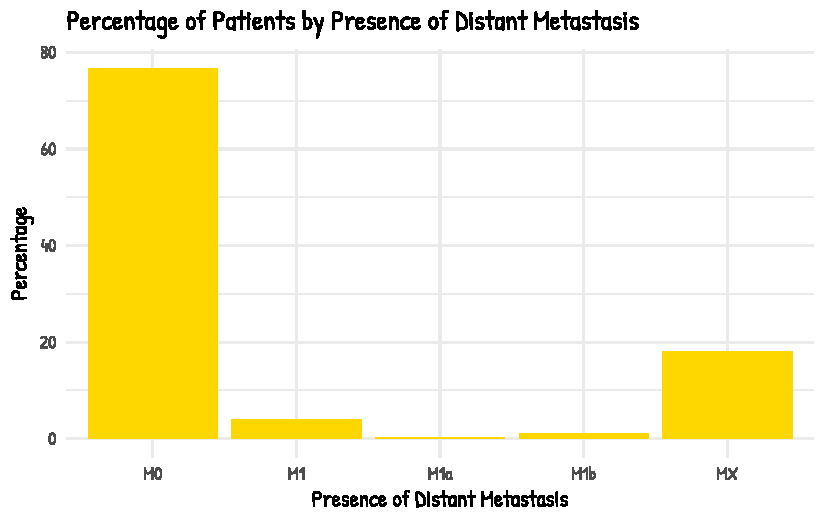
\includegraphics{paper_files/figure-pdf/fig-bills-3.pdf}

}

\caption{\label{fig-bills-3}bb}

\end{figure}

\begin{figure}

{\centering 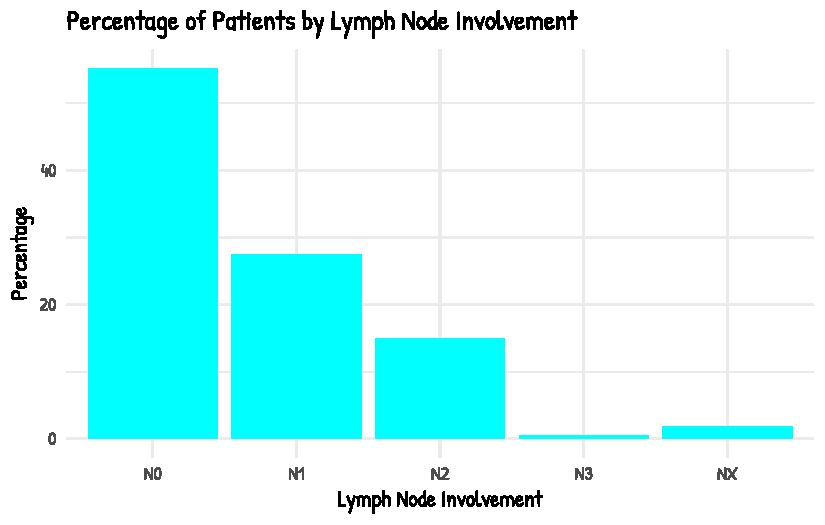
\includegraphics{paper_files/figure-pdf/fig-bills-4.pdf}

}

\caption{\label{fig-bills-4}bb}

\end{figure}

\begin{figure}

{\centering 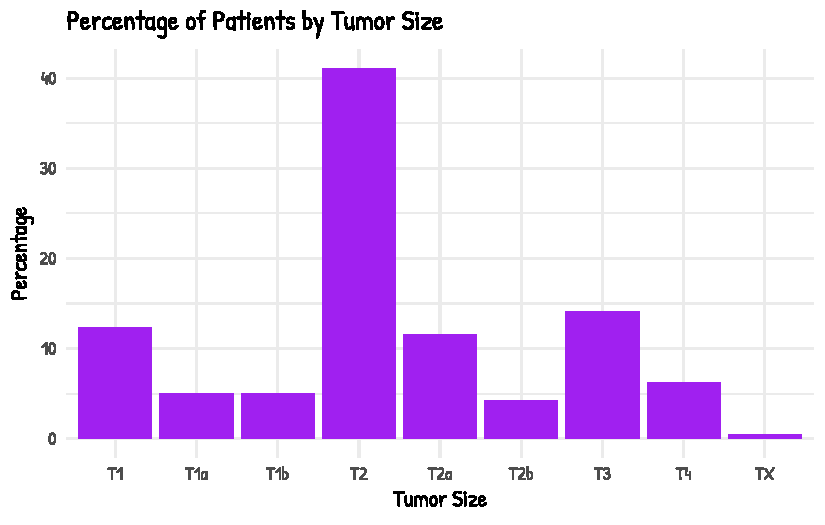
\includegraphics{paper_files/figure-pdf/fig-bills-5.pdf}

}

\caption{\label{fig-bills-5}bb}

\end{figure}

\begin{figure}

{\centering 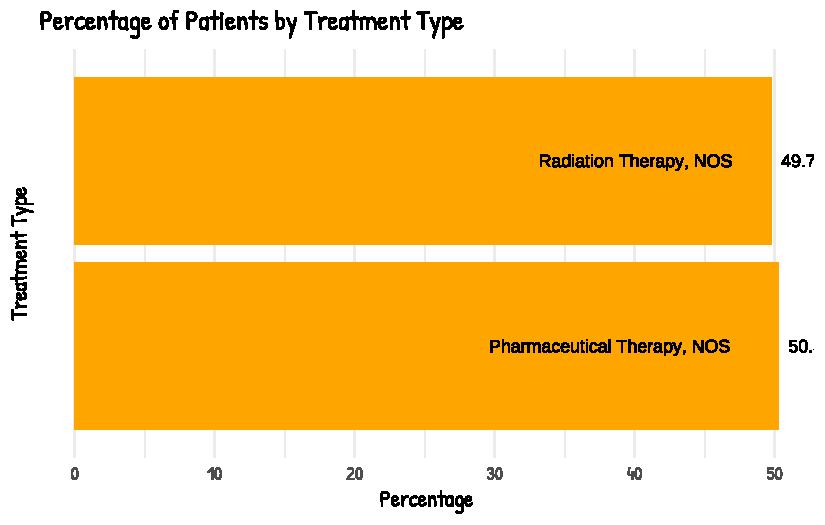
\includegraphics{paper_files/figure-pdf/fig-bills-6.pdf}

}

\caption{\label{fig-bills-6}bb}

\end{figure}

Talk more about it.

\hypertarget{sec-model}{%
\section{Model}\label{sec-model}}

\hypertarget{model-set-up}{%
\subsection{Model set-up}\label{model-set-up}}

In this section, we aim to predict the survival outcomes of lung cancer
patients post-diagnosis with a linear regression model framework. We
consider several predictors including pathogenic stage, lymph node
involvement, presence of distant metastasis, tumor size, and treatment
type.We specify the model and subsequently justify its appropriateness
for our analysis.

\hypertarget{model-specifications}{%
\subsubsection{Model Specifications}\label{model-specifications}}

We employ a linear regression model to predict the number of days from
diagnosis to death for each lung cancer patient. The model is defined as
follows:

\(y_i\) \textbar{} \mu\_i, \sigma \&\sim \text{Normal}(\mu\_i, \sigma)

where: * \(y_i\) represents the number of days from diagnosis to death
for patient \(i\). * \(mu_i\) denotes the expected number of days to
death for patient \(i\). * \(σ\) represesents the standard deviation of
the survival times.

The linear predictor \(mu_i\) is specified as:

\mu\emph{i = \alpha + \beta}\{\text{pathologic_stage}\}
\times \text{pathologic_stage}\emph{i + \beta}\{\text{lymph_node}\}
\times \text{lymph_node_involvement}\emph{i +
\beta}\{\text{metastasis}\}
\times \text{presence_of_distant_metastasis}\emph{i +
\beta}\{\text{tumor_size}\} \times \text{tumor_size}\emph{i +
\beta}\{\text{treatment_type}\} \times \text{treatment_type}\_i

where:

\begin{itemize}
\tightlist
\item
  \alpha represents the intercept term, capturing the baseline number of
  days to death.
\item
  \beta\emph{\{\text{pathologic_stage}\}, \beta}\{\text{lymph_node}\},
  \beta\emph{\{\text{metastasis}\}, \beta}\{\text{tumor_size}\},
  \beta\_\{\text{treatment_type}\} are the coefficients associated with
  each predictor variable.
\end{itemize}

\hypertarget{model-justification}{%
\subsubsection{Model justification}\label{model-justification}}

Linear regression models are most appropritate in predicting continuous
outcomes. As survival time is continuous, this model allows us to
quantify the relationships between these predictors and survival
outcomes, providing valuable insights into the factors influencing the
prognosis of lung cancer patients.

\hypertarget{response-variable}{%
\paragraph{Response Variable}\label{response-variable}}

Out variable of interest is survival time in lung cancer patient afte
they have been diagnosed

We model the survival time (\(y_i\)) as a continuous variable,
reflecting the duration from diagnosis to death for each patient. This
continuous characterization is appropriate for capturing the temporal
aspect of survival outcomes in medical contexts.

\hypertarget{input-variables}{%
\paragraph{Input Variables}\label{input-variables}}

We consider several clinically relevant predictors including pathologic
stage, lymph node involvement, presence of distant metastasis, tumor
size, and treatment type. These variables are chosen based on their
established associations with lung cancer prognosis, encompassing key
aspects of disease severity and treatment strategies.

\hypertarget{model-structure}{%
\paragraph{Model Structure}\label{model-structure}}

The linear regression model relates the expected survival time (\(μ_i\))
to the linear combination of predictor variables, allowing us to
quantify the impact of each predictor on the expected duration of
survival. This framework facilitates interpretation of the associations
between clinical variables and survival outcomes, providing valuable
insights for patient prognosis.

\hypertarget{parameter-estimation}{%
\paragraph{Parameter Estimation}\label{parameter-estimation}}

We anticipate that the survival time of lung cancer patients
post-diagnosis will be influenced by various clinical factors such as
pathologic stage, extent of lymph node involvement, presence of distant
metastasis, tumor size, and treatment type. Specifically, we expect that
advanced pathologic stages, increased lymph node involvement, presence
of distant metastasis, larger tumor sizes, and certain treatment types
will be associated with shorter survival times.

We run the model in R (R Core Team 2023) estimating the model
coefficients (\(/alpha\) and \(/beta\)) using Bayesian inference via the
`stan\_glm()' function from the Goodrich et al. (2022) package. This
approach leverages Markov Chain Monte Carlo (MCMC) algorithms to obtain
posterior distributions for the model parameters, enabling robust
estimation of parameter uncertainties and inference on the effects of
predictor variables.

\hypertarget{sec-results}{%
\section{Results}\label{sec-results}}

Our results are summarized in @.

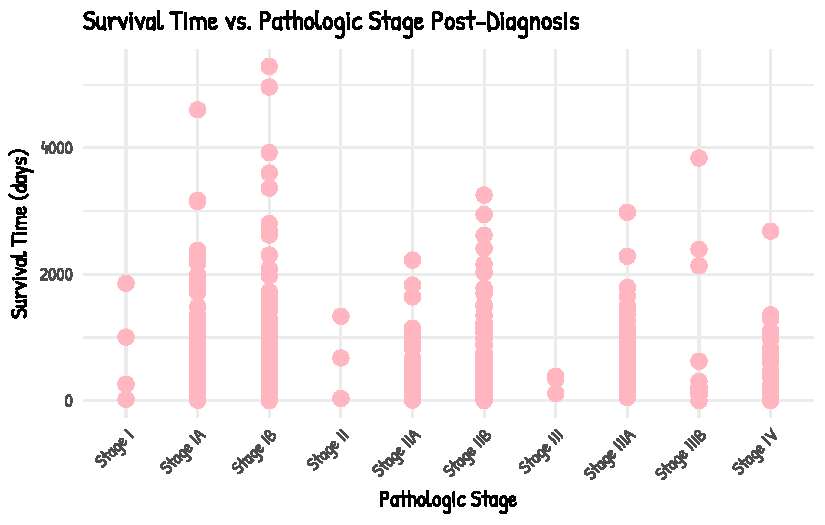
\includegraphics{paper_files/figure-pdf/unnamed-chunk-4-1.pdf}

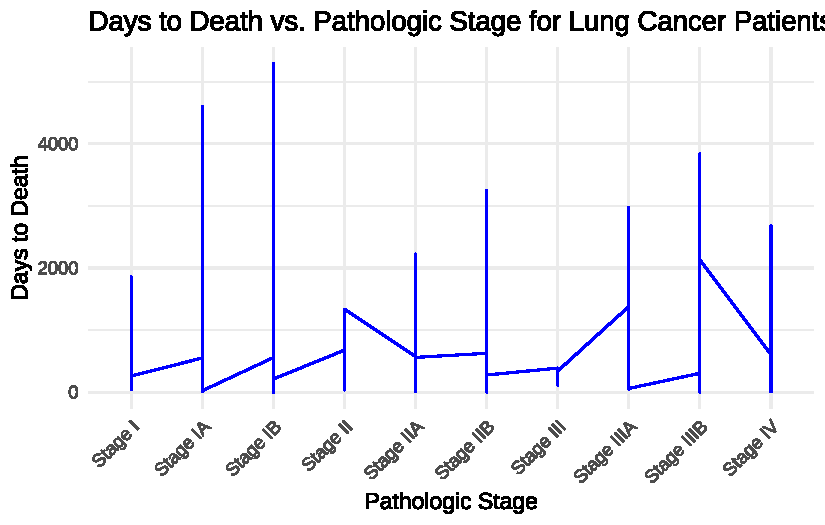
\includegraphics{paper_files/figure-pdf/unnamed-chunk-4-2.pdf}

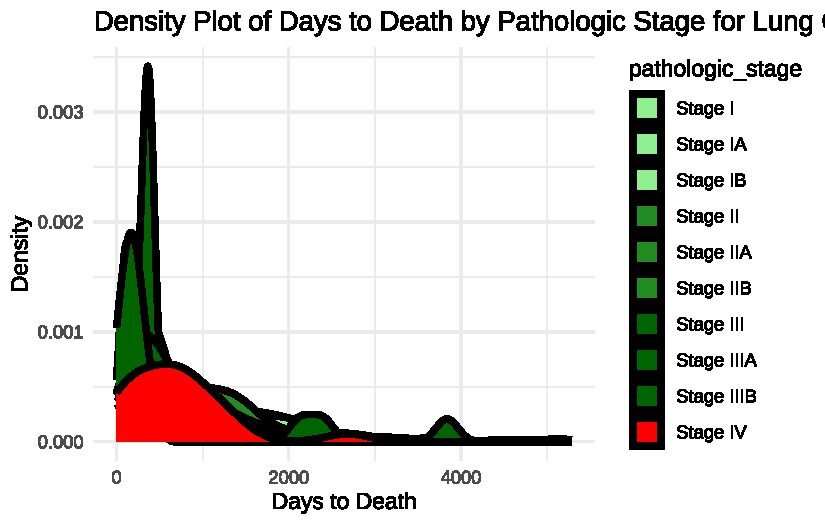
\includegraphics{paper_files/figure-pdf/unnamed-chunk-4-3.pdf}

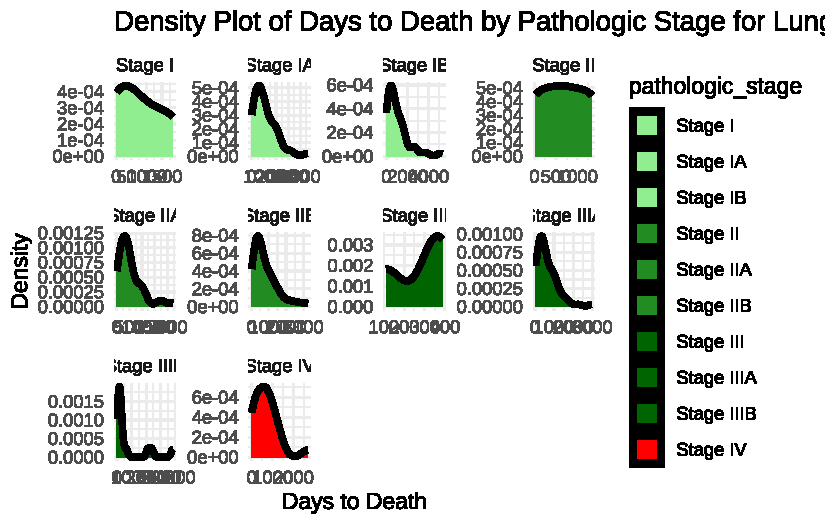
\includegraphics{paper_files/figure-pdf/unnamed-chunk-4-4.pdf}

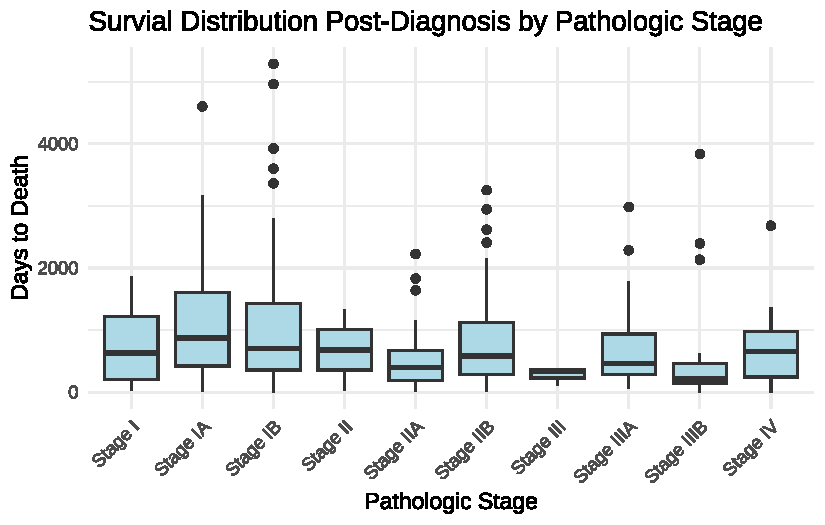
\includegraphics{paper_files/figure-pdf/unnamed-chunk-4-5.pdf}

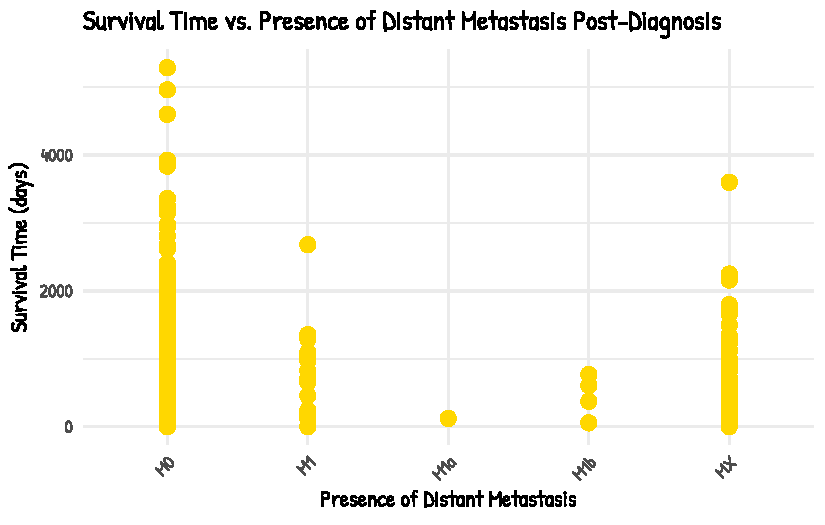
\includegraphics{paper_files/figure-pdf/unnamed-chunk-4-6.pdf}

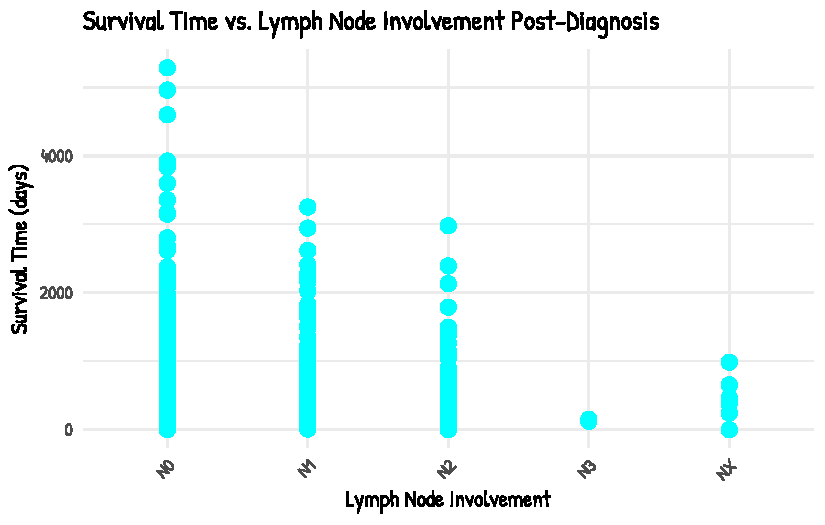
\includegraphics{paper_files/figure-pdf/unnamed-chunk-4-7.pdf}

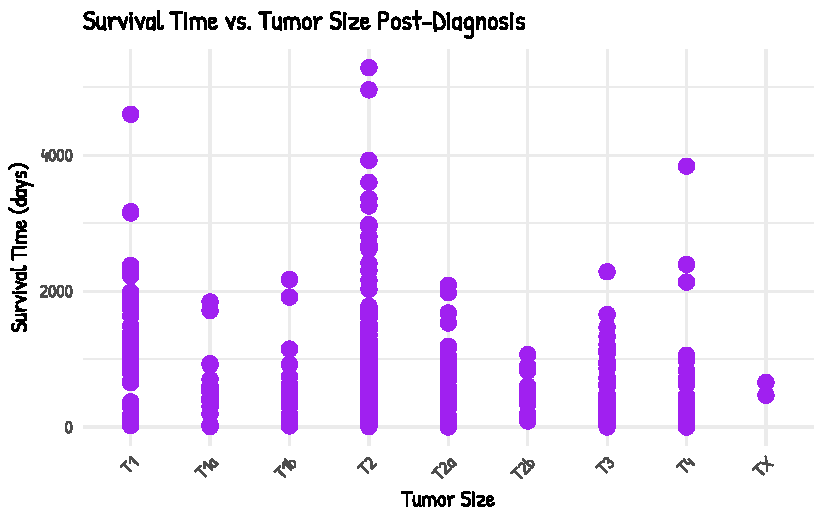
\includegraphics{paper_files/figure-pdf/unnamed-chunk-4-8.pdf}

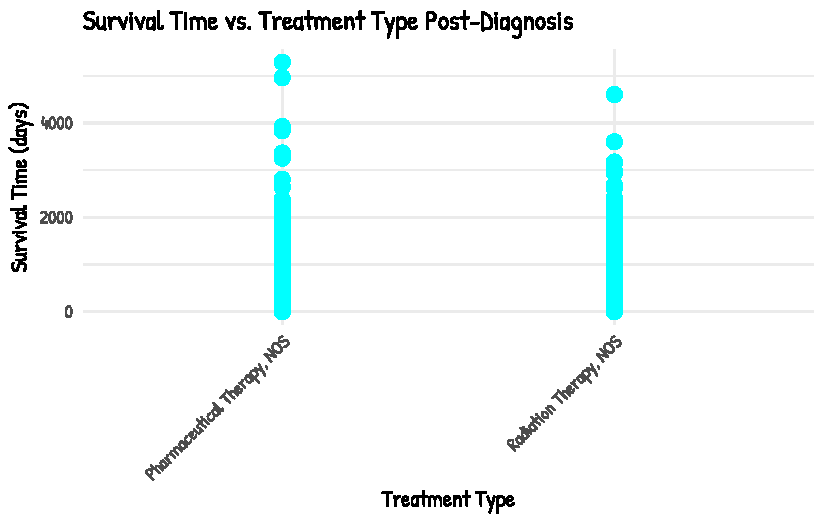
\includegraphics{paper_files/figure-pdf/unnamed-chunk-4-9.pdf}

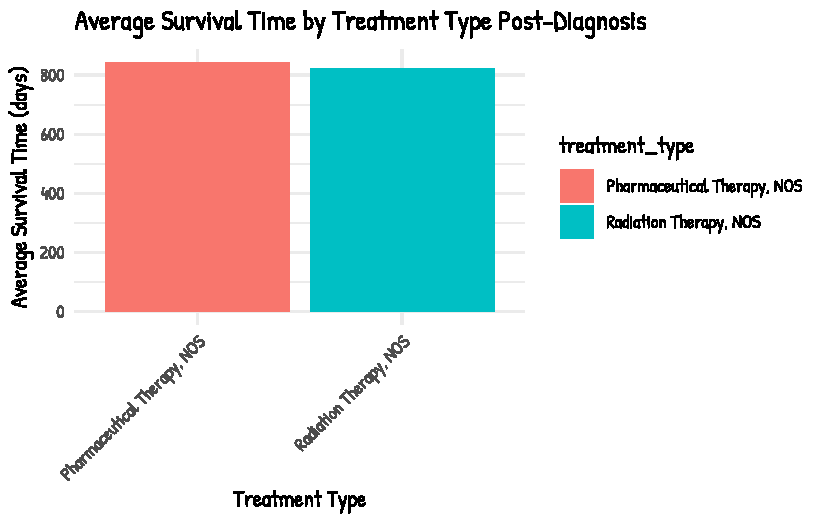
\includegraphics{paper_files/figure-pdf/unnamed-chunk-4-10.pdf}

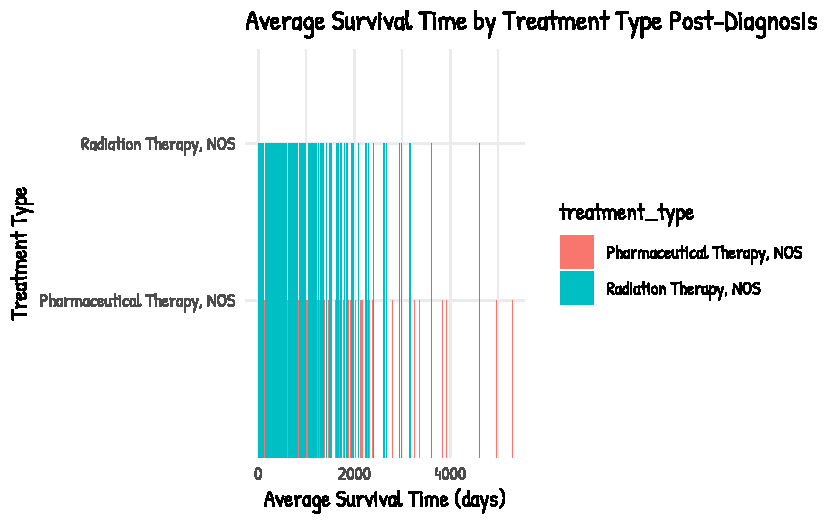
\includegraphics{paper_files/figure-pdf/unnamed-chunk-4-11.pdf}

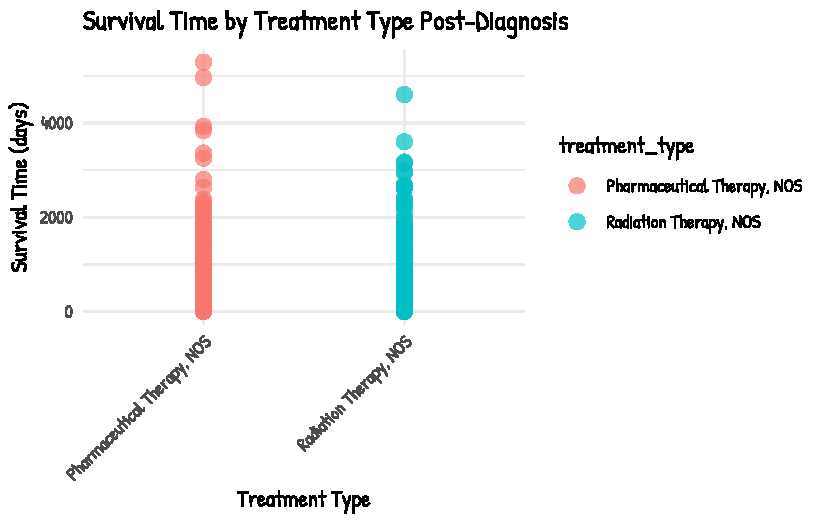
\includegraphics{paper_files/figure-pdf/unnamed-chunk-4-12.pdf}

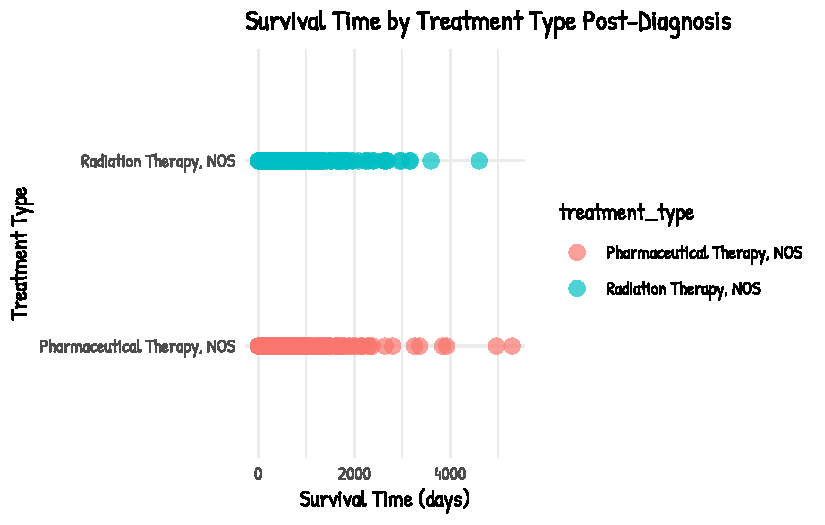
\includegraphics{paper_files/figure-pdf/unnamed-chunk-4-13.pdf}

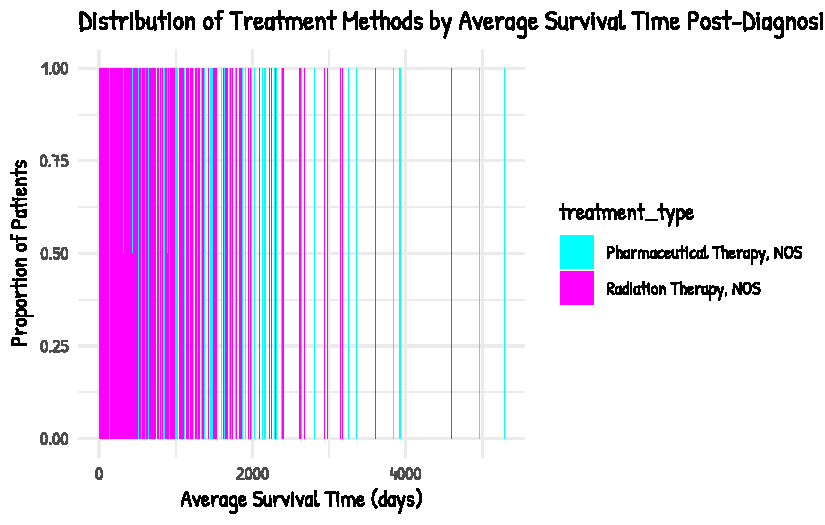
\includegraphics{paper_files/figure-pdf/unnamed-chunk-4-14.pdf}

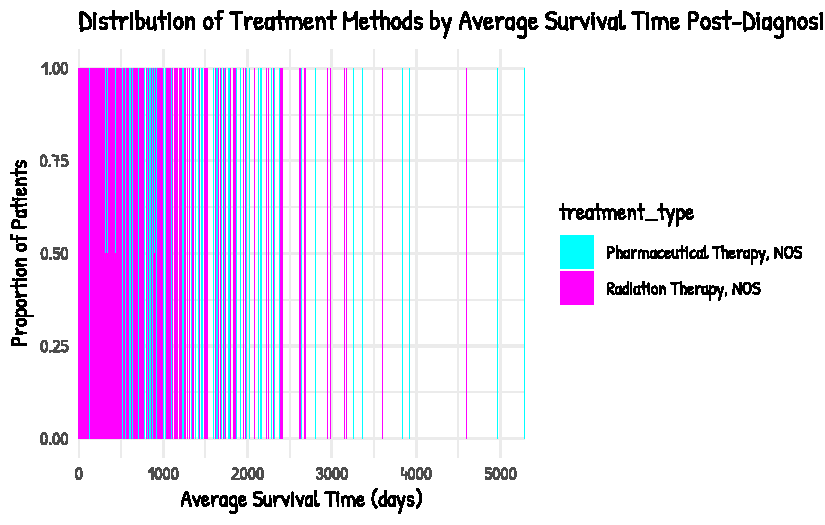
\includegraphics{paper_files/figure-pdf/unnamed-chunk-4-15.pdf}

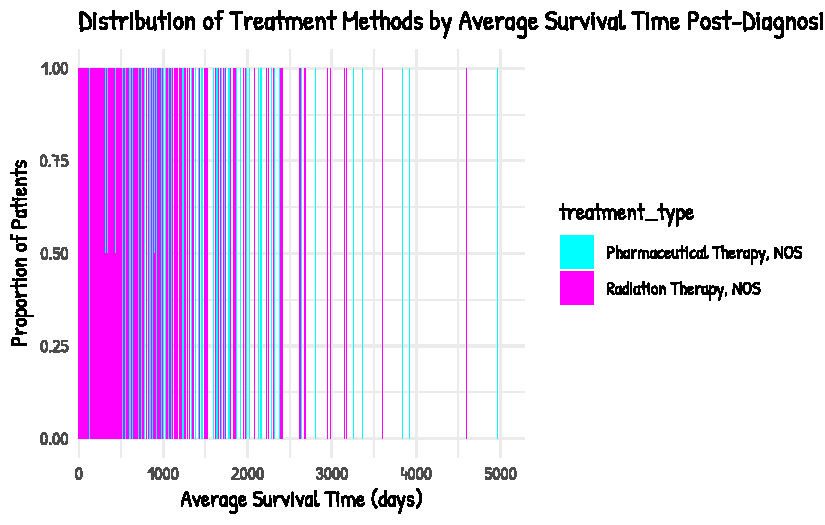
\includegraphics{paper_files/figure-pdf/unnamed-chunk-4-16.pdf}

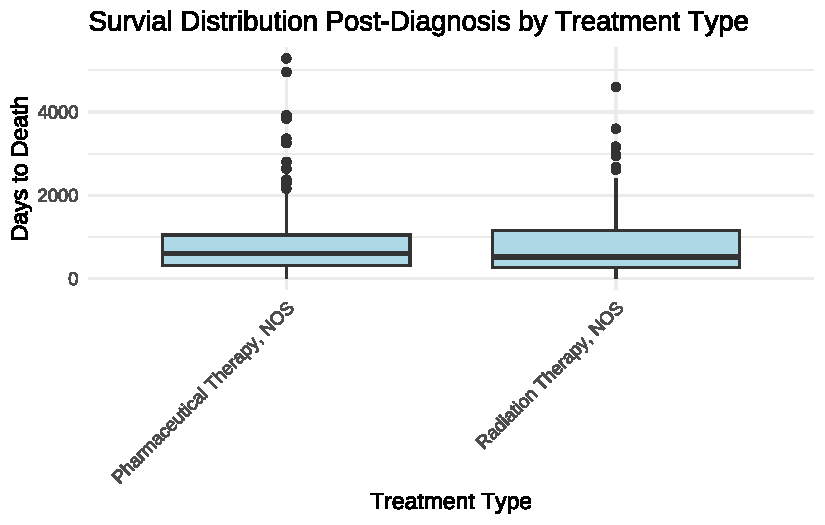
\includegraphics{paper_files/figure-pdf/unnamed-chunk-4-17.pdf}

\begin{table}

\end{table}

\hypertarget{sec-discussion}{%
\section{Discussion}\label{sec-discussion}}

\hypertarget{sec-first-point}{%
\subsection{First discussion point}\label{sec-first-point}}

\hypertarget{second-discussion-point}{%
\subsection{Second discussion point}\label{second-discussion-point}}

\hypertarget{third-discussion-point}{%
\subsection{Third discussion point}\label{third-discussion-point}}

\hypertarget{weaknesses-and-next-steps}{%
\subsection{Weaknesses and next steps}\label{weaknesses-and-next-steps}}

\newpage

\appendix

\hypertarget{sec-appendix}{%
\section{Appendix}\label{sec-appendix}}

\hypertarget{additional-data-details}{%
\section{Additional data details}\label{additional-data-details}}

\hypertarget{sec-model-details}{%
\section{Model details}\label{sec-model-details}}

we compare the posterior with the prior. This shows\ldots{}

\begin{figure}

\begin{minipage}[t]{0.50\linewidth}

{\centering 

Examining how the model fits, and is affected by, the data

}

\end{minipage}%

\caption{\label{fig-ppcheckandposteriorvsprior}\textbf{?(caption)}}

\end{figure}

\hypertarget{diagnostics}{%
\subsection{Diagnostics}\label{diagnostics}}

Is this needed?

\begin{figure}

\begin{minipage}[t]{0.50\linewidth}

{\centering 

Checking the convergence of the MCMC algorithm

}

\end{minipage}%

\caption{\label{fig-stanareyouokay}\textbf{?(caption)}}

\end{figure}

\newpage

\hypertarget{references}{%
\section*{References}\label{references}}
\addcontentsline{toc}{section}{References}

\hypertarget{refs}{}
\begin{CSLReferences}{1}{0}
\leavevmode\vadjust pre{\hypertarget{ref-rstanarm}{}}%
Goodrich, Ben, Jonah Gabry, Imad Ali, and Sam Brilleman. 2022.
{``Rstanarm: {Bayesian} Applied Regression Modeling via {Stan}.''}
\url{https://mc-stan.org/rstanarm/}.

\leavevmode\vadjust pre{\hypertarget{ref-citeR}{}}%
R Core Team. 2023. \emph{R: A Language and Environment for Statistical
Computing}. Vienna, Austria: R Foundation for Statistical Computing.
\url{https://www.R-project.org/}.

\end{CSLReferences}



\end{document}
